\documentclass{article}
\usepackage{amssymb}
\usepackage{mathtools}
\usepackage{amsmath}
\usepackage{hyperref}
\usepackage{setspace}
\usepackage[utf8]{inputenc}
 
\usepackage{listings}
\usepackage{color}
\usepackage{graphicx}
\usepackage[english]{babel}
 
\setlength{\parindent}{4em}
\setlength{\parskip}{1em}
 
\definecolor{codegreen}{rgb}{0,0.6,0}
\definecolor{codegray}{rgb}{0.5,0.5,0.5}
\definecolor{codepurple}{rgb}{0.58,0,0.82}
\definecolor{backcolour}{rgb}{0.95,0.95,0.92}
 
\lstdefinestyle{mystyle}{
    backgroundcolor=\color{backcolour},   
    commentstyle=\color{codegreen},
    keywordstyle=\color{magenta},
    numberstyle=\tiny\color{codegray},
    stringstyle=\color{codepurple},
    basicstyle=\footnotesize,
    breakatwhitespace=false,         
    breaklines=true,                 
    captionpos=b,                    
    keepspaces=true,                 
    numbers=left,                    
    numbersep=5pt,                  
    showspaces=false,                
    showstringspaces=false,
    showtabs=false,                  
    tabsize=2
}

\newcommand{\norm}[1]{\left\lVert#1\right\rVert}
 
\lstset{style=mystyle}

\everymath{\displaystyle}

\begin{document}

\raggedright

\doublespacing


\title{ {\Huge{Data Mining 2015 - Homework 2}} }
\author {Ludovico Fabbri 1197400}
\maketitle


\section{Problem 1}
Here we are asking to implement nearest-neighbor search for text documents. You have to implement shingling, minwise hashing, and locality-sensitive hashing. 

\subsection{}
Implement a class that, given a document, creates its set of character shingles of some length k. Then represent the document as the set of the hashes of the shingles, for some hash function.

\begin{lstlisting} 
from Helpers import *

class ShingleDocument:
    def __init__(self, doc, shingleSize):
        self.shingles = set()

        if len(doc) <= shingleSize:
            return doc

        # sequences of two or more white spaces will be normalized to one white space
        docProcessed = normalizeWhiteSpaces(doc)

        for i in range(0, len(docProcessed) - (shingleSize-1)):
            shingle = docProcessed[i:i+shingleSize]
            hashedShingle = hash(shingle)
            self.shingles.add(hashedShingle)
\end{lstlisting}

Simple class with an attribute of type set named 'shingles' where are stored the hashes of the shingles for that document object. The built in set in python assures that duplicates of shingles are discarded. Before computing the shingles, there is an helper function from Helper.py that normalizes white spaces in a preprocessing step.



\subsection{}
Implement a class, that given a collection of sets of objects (e.g., strings, or numbers), creates a minwise hashing based signature for each set.

\begin{lstlisting} 
from Helpers import *

class MinHashSets:
    def __init__(self, collectionShigleDocs, n):

        # Dictionary (key=index of document, value=signature of the document)
        self.minHashSets = {}

        # Generating minhash family functions
        hashFunctions = []
        for i in range(n):
            hashFunctions.append(hashFamily(i))

        # LSH alg
        i = 0
        for shingleDoc in collectionShigleDocs:
            j = 0
            for hashFunc in hashFunctions:
                shingles = set()
                for shingle in shingleDoc.shingles:
                    shingles.add(hashFunc(str(shingle)))

                if j == 0:
                    self.minHashSets[i] = [min(shingles)]
                else:
                    self.minHashSets[i].append(min(shingles))
                j = j + 1
            i = i + 1
\end{lstlisting}

The dictionary 'minHashSets' stores the signature for each document. After generating a family of n minhash functions we start the minhash algorithm generating the signature for each document.




\subsection{}
Implement a class that implements the locally sensitive hashing (LSH) technique, so that, given a collection of minwise hash signatures of a set of documents, it finds the all the documents pairs that are near each other.

\begin{lstlisting} 
class LSH:
    def __init__(self, minHashSets, numBands, bandWidth, n):

        self.bandsArray = []
        self.candidatePairs = []
        self.nearDuplicates = set()

        start = 0
        for b in range(numBands):
            newDic = {}
            self.bandsArray.append(newDic)
            if (b != 0):
                start += bandWidth

            for key in minHashSets:
                signature = minHashSets[key]
                sliceSignature = signature[start:start+bandWidth]
                sliceSignatureConcat = ""

                for minhash in sliceSignature:
                    sliceSignatureConcat += minhash
                    currentDictionary = self.bandsArray[b]
                hashBucketKey = hash(sliceSignatureConcat)

                if not currentDictionary.has_key(hashBucketKey):
                    currentDictionary[hashBucketKey] = []
                    currentDictionary[hashBucketKey].append(key)
                else:
                    for documentKey in currentDictionary[hashBucketKey]:
                        candidatePair = (key,documentKey)
                        self.candidatePairs.append(candidatePair)
                    currentDictionary[hashBucketKey].append(key)

        # remove symmetric pairs
        self.candidatePairs = set((a,b) if a<=b else (b,a) for a,b in self.candidatePairs)

        # select near-duplicates
        for candidatePair in self.candidatePairs:
            duplicateKey = candidatePair[1]
            self.nearDuplicates.add(duplicateKey)
\end{lstlisting}

In this class there 3 attributes: 
\begin{itemize}
	\item bandsArray: for each band stores a dictionary of the candidate-pairs
	\item candidatePairs: a list of all the candidate pairs found by the lsh algorithm
	\item nearDuplicates: a set of all the near-duplicates found by the lsh algorithm
\end{itemize}

For each band we iterate over signatures and slice each signature to the width of a band (r). We hash this slice-signature to a bucket (the key of the dictionary) and append the document index to the list related to that key. We have to remove symmetric pairs (example (1,2) and (2,1)) before computing near-duplicates documents, which we do in the last step.


\subsection{}
To test the LSH algorithm, also implement a class that given the shingles of each of the docu- ments, finds the nearest neighbors by comparing all the shingle sets with each other.

\begin{lstlisting}
from Helpers import jaccardSim

class ShingleSimilarity:
    def __init__(self,shingleDocuments):

        self.neighboursPairs = set()
        self.nearDuplicates = set()

        for i in range(len(shingleDocuments)):
            shingleDoc1 = shingleDocuments[i]
            for j in range (i+1, len(shingleDocuments)):
                #if (j != i):
                shingleDoc2 = shingleDocuments[j]
                if jaccardSim(shingleDoc1.shingles, shingleDoc2.shingles) >= 0.8:
                    pair = (i,j)
                    self.neighboursPairs.add(pair)

        # remove symmetric pairs
        self.neighboursPairs = set((a,b) if a<=b else (b,a) for a,b in self.neighboursPairs)

        # select near-duplicates
        for pair in self.neighboursPairs:
            duplicateKey = pair[1]
            self.nearDuplicates.add(duplicateKey)
\end{lstlisting}

This class simply use an helper method to compute Jaccard similarity between each set of shingles and the others set, selecting only them that have an index of similarity greater than 0.8.
There are 2 attributes:
\begin{itemize}
	\item neighboursPairs: a set of the pairs of the near-duplicates
	\item nearDuplicates: a set of the near-duplicates
\end{itemize}



\subsection{}
Here the file that implements the helpers methods:

\begin{lstlisting}
import hashlib
import re

# regular expression for one or more tabs
spacesRE = re.compile("\s+")


# Format a text document converting the sequences of two ore more whitespaces in one whitespace
def normalizeWhiteSpaces(doc):
    result = re.sub(spacesRE, " ", doc);
    return result


# Implement a family of hash functions. It hashes strings and takes an # integer to define the member of the family.
# Return a hash function parametrized by i
def hashFamily(i):
    resultSize = 8      # how many bytes we want back
    maxLen = 20         # how long can our i be (in decimal)
    salt = str(i).zfill(maxLen)[-maxLen:]
    def hashMember(x):
        hasher = hashlib.sha1(x + salt).digest()[-resultSize:]
        return hasher
    return hashMember


# Jaccard Similarity
def jaccardSim(shingles1, shingles2):
    intersection = len(set(shingles1).intersection(shingles2))
    return intersection / float(len(shingles1) + len(shingles2) - intersection)
\end{lstlisting}



\subsection{}
This is the main program, where there is computational time for each step of the problem, the number of near duplicates found using LSH and Jaccard similarity respectively and the size of the intersection.
For the input i am using output file of the first homework (problem6output.tsv) and selecting each long description as the document.
\begin{lstlisting}
#!/usr/bin/env python

from ShingleDoc import ShingleDocument
from MinHash import MinHashSets
from LSH import LSH
from ShingleSimilarity import ShingleSimilarity
import time

print""
print ("START")

k = 10      # shingle size
n = 100     # number of permutations (minhash functions)
b = 10      # number of bands
r = 10      # number of rors for band (bandridth)

print""
print " ------------------------ "
print "Shingle size: " + str(k)
print "Number of minhash permutations: " + str(n)
print "Number of bands: " + str(b)
print "Number of rors for band: " + str(r)
print " ------------------------ "
print""


file = open("problem6output.tsv", 'r')
jobs = file.read().split('\n')
file.close()

shingleDocuments = []
end = len(jobs)-1



print "Computing shingles..."
start = time.time()
for i in range(0, end):
    job = jobs[i]
    jobDescription = job.split('\t')[5]
    shingleDoc = ShingleDocument(jobDescription, k)
    shingleDocuments.append(shingleDoc)
shiglesTime = time.time() - start
print "DONE. Time: " + str(shiglesTime)


print""
print " ------------------------ "
print""


print "Computing minhashings..."
minhashingTimeStart = time.time()
minHashSets = MinHashSets(shingleDocuments, n).minHashSets
minhashingTimeEnd = time.time() - minhashingTimeStart
print "DONE. Time: " + str(minhashingTimeEnd)
#for key in minHashSets:
#    print len(minHashSets[key]), minHashSets[key]


print""
print " ------------------------ "
print""


print "Computing LSH..."
lshTimeStart = time.time()
lsh = LSH(minHashSets, b, r, n)
lshTimeEnd = time.time() - lshTimeStart
print "DONE. Time: " + str(lshTimeEnd)
candidatePairs = lsh.candidatePairs
nearDuplicatesLSH = lsh.nearDuplicates
print "Number of pairs: " + str(len(candidatePairs))
print "Number of duplicates: " + str(len(nearDuplicatesLSH))


print""
print " ------------------------ "
print""


print "Computing Jaccard Similarity..."
jaccartTimeStart = time.time()
shingleSimilarity = ShingleSimilarity(shingleDocuments)
jaccartTimeEnd = time.time() - jaccartTimeStart
print ("DONE. Time: " + str(jaccartTimeEnd))
neighboursPairs = shingleSimilarity.neighboursPairs
nearDuplicatesJS = shingleSimilarity.nearDuplicates
#print shingleSimilarity.neighboursPairs
#print shingleSimilarity.nearDuplicates
print "Number of pairs: " + str(len(neighboursPairs))
print "Number of duplicates: " + str(len(nearDuplicatesJS))


print""
print " ------------------------ "
print""

print "Intersection between Jaccard and LSH near-duplicates: " + str(len(set(nearDuplicatesJS).intersection(nearDuplicatesLSH)))


print""
print "END"\end{lstlisting}


\newpage


To find the right values for b and r i've used Wolfram, with n fixed at 100 and the thereshold t=0.8 \\
\begin{figure} [h]
\centering
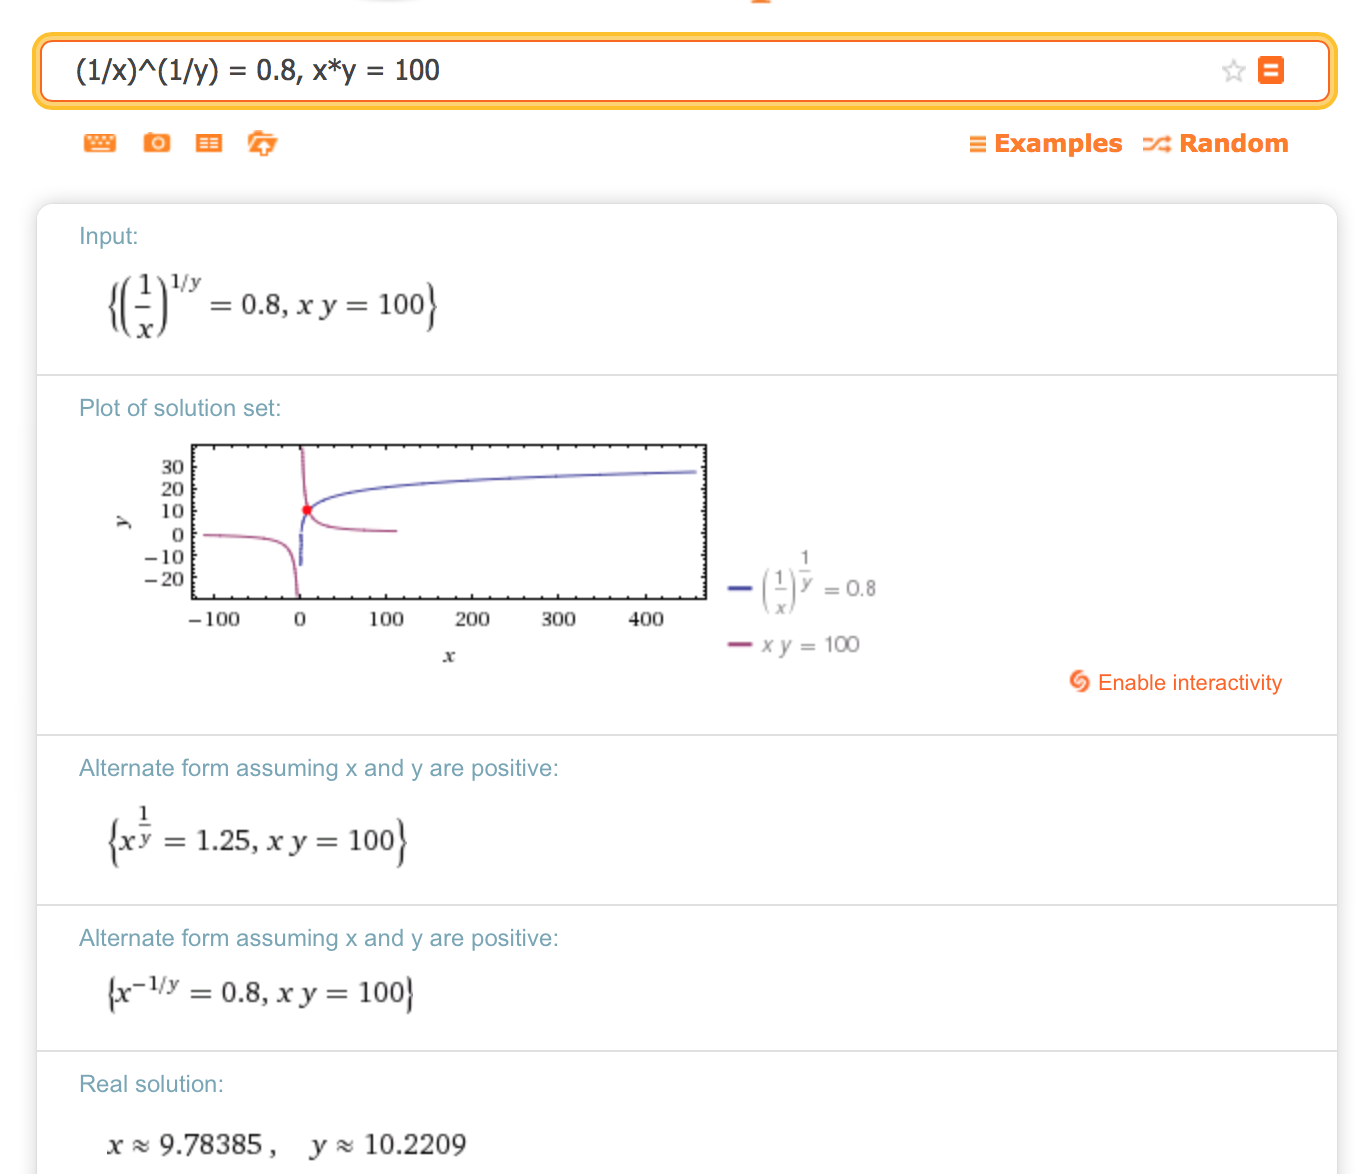
\includegraphics[width=150mm]{wolfram1010}
\caption{Wolfram computing b and r in LSH with n=100 and t=0.8  \label{wolfram1}}
\end{figure}

So i've choose b=10 and r=10. \\


\newpage

And this is the output of the whole program: \\

\begin{figure} [h]
\centering
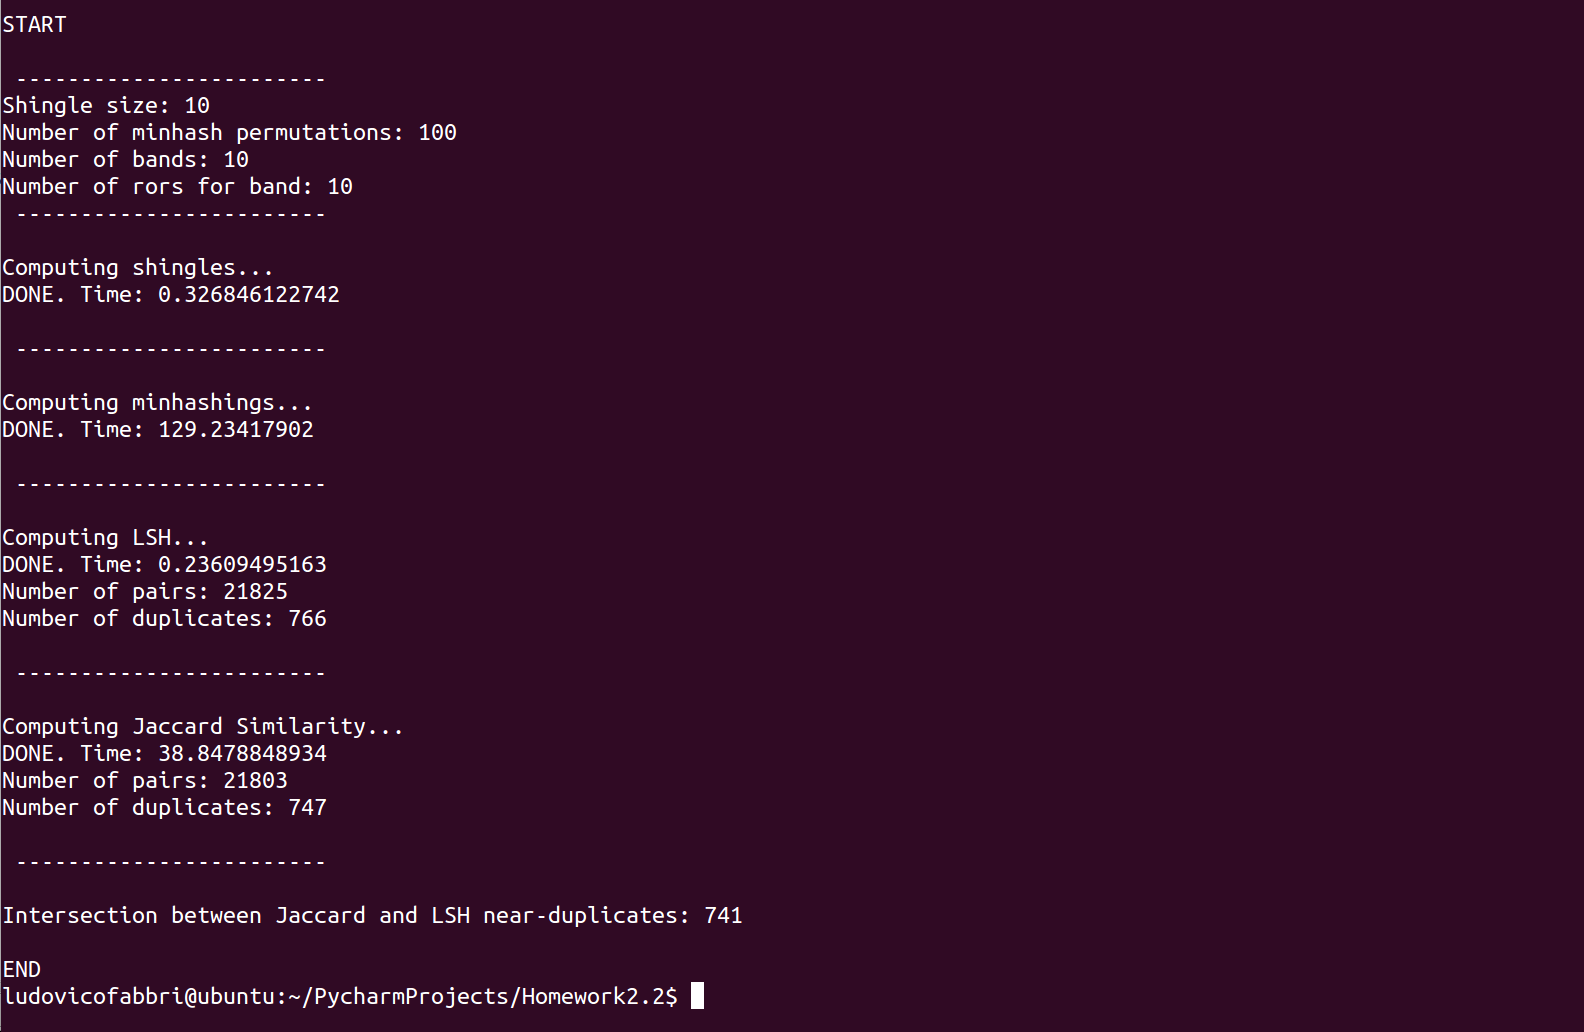
\includegraphics[width=150mm]{output1010}
\caption{output for n=100, b=10, r=10, t=0.794  \label{wolfram1}}
\end{figure}

\begin{itemize}
	\item Time of LSH: 0.236
	\item Number of near-duplicates found with LSH: 766
	\item Time of Jaccard similarity: 38.847
	\item Number of near-duplicates found with JS: 747
	\item Size of the intersection: 741
\end{itemize}







\section{Problem 2}


\subsection{}
Recall that the k-means cost function for clustering C is the:

\begin{equation} \label{eq:objective_kmeans}
J = \sum_{k=1}^{K}  \sum_{x_{i} \in C_{k}}  \norm { x_{i} - \mu_{k} }^{2}_{2}
\end{equation}

where $C = \left\{ C_{1}, C_{2}, ... , C_{k}   \right\}$ is a clustering of the dataset V.

We want to minimize the $l_{1}$ distance between points of the dataset and the relative cluster center in this objective function:

\begin{equation} \label{eq:objectiveFunc1}
J = \sum_{k=1}^{K}  \sum_{x_{i} \in C_{k}}  \norm { x_{i} - \mu_{k} }_{1}
\end{equation}

where K is the set of clusters, $x_{i}$ are the points of dataset and $\mu_{k}$ are the centroids of clusters. We can re-write this function in another way:

\begin{equation} \label{eq:objectiveFunc2}
J = \sum_{n=1}^{N}  \sum_{k=1}^{K} r_{nk} \cdot \norm{ x_{i} - \mu_{k} }_{1}
\end{equation}

Where N is the set of points of the dataset and  $r_{nk}$ is a binary indicator variable defined as follow:

\begin{equation} \label{eq:rnk}
r_{nk} = 
\begin{cases}
	1 & \text{ if the n-th point is assigned to the k-th cluster} \\
	0 & \text{ otherwise } \\
\end{cases}
\end{equation}

Our goal is to find values for $ \left\{r_{nk} \right\} $ and $ \left\{ \mu_{k} \right\} $ that minimize J. \\
To do this we can use an iterative approach in which each iteration is divided in two successive steps:
\begin{enumerate}
	\item First we optimize $x_{n}$ keeping $\mu_{k}$ fixed 
	\item Than we optimize $\mu_{k}$ keeping $x_{n}$ fixed
\end{enumerate}

We can repeat this procedure until convergence for some threshold parameter. \\

In the first step we have centroids fixed and want to minimize J as function of the distribution of the point $x_{n}$, that is find $r_{nk}$. 
Since each point of the dataset is independent from the others, we can choose $r_{nk}$ to minimize the manhattan distance (norm-1 distance or $l_{1}$)
between the point $x_{n}$ and the centroid $\mu_{k}$. So we have that:

\begin{equation} \label{eq:rnk_norm1}
r_{nk} = 
\begin{cases}
	1 & \text{ if k = arg $min_{j}  \norm{x_{n} - \mu_{j}}_{1}  $} \\
	0 & \text{ otherwise } \\
\end{cases}
\end{equation}


Because we are in an ordinated space (otherwise manhattan distance has no sense), assuming that $\rho(x_{1}, \mu_{1})$ is the manhattan distance between the point $x_{1}$ and the centroid $\mu_{1}$ and
$\rho(x_{1}, \mu_{2})$ is the distance between the same point and the centroid centroid $\mu_{2}$, we can say that if $\rho(x_{1}, \mu_{1}) < \rho(x_{1}, \mu_{2})$, than also the euclidean distance (2-norm or $l_{2}$) between 
point $x_{1}$ and the centroid $\mu_{1}$ is lower than the euclidean distance between $x_{1}$ and the centroid $\mu_{2}$. That is, we can re-write $r_{nk}$ using the $l_{2}$ euclidean distance:

\begin{equation} \label{eq:rnk_norm1}
r_{nk} = 
\begin{cases}
	1 & \text{ if k = arg $min_{j}  \norm{x_{n} - \mu_{j}}_{2}  $} \\
	0 & \text{ otherwise } \\
\end{cases}
\end{equation}

So far, we found that the first step of the optimization algorithm will find the same $r_{nk}$ using the objective function of k-means in the (\ref{eq:objective_kmeans}) which uses the 2-norm distance or the objective function in the (\ref{eq:objectiveFunc1}) which uses the 1-norm distance.\\

Now let's focus on the second step. We want to find values for centroids $\mu_{k}$ that minimize J keeping $r_{nk}$ fixed (so the data points are assigned). 
So we want to resolve this problem:

\begin{equation} \label{eq:objectiveFunc3}
min( \sum_{n=1}^{N} r_{nk} \cdot  \norm { x_{n} - \mu_{k} }_{1})      \;\;\;\;\;\;\;\;\;\;\;      \forall k \in K
\end{equation}

To find the minimum we can calculate the derivative of the function above with respect to $\mu_{k}$ and set it equal to zero. We know that the derivative of the absolute value is the sign function (excluding the point where argument is zero). 
That is:

\begin{equation} \label{eq:derivative1Func3}
\frac {\partial J} {\partial \mu_{k}}	=	\frac {\partial \sum_{n=1}^{N} r_{nk} \cdot \norm { x_{n} - \mu_{k} }_{1}} {\partial \mu_{k}}		= 0
\end{equation}

\begin{equation} \label{eq:derivative2Func3}
\frac {\partial J} {\partial \mu_{k}}	=		\sum_{n=1}^{N} {r_{nk} \cdot sign(x_{n} - \mu_{k})} 	= 0		\;\;\;\;\;\;\;\;\;\;\;      \forall k \in K, \mu_{k} \neq x_{n}
\end{equation}

So for each cluster we want to find $\mu_{k}$ that makes a partition for that cluster such that we will have the sum of the sign functions equal to zero.
Among the infinite solutions we can find, we want to find the one that minimize the absolute error between the data-points of the cluster.
We can recall a well known property of the median, which is to minimize the sum of the mean absolute errors of a set of values $x_{i}$ from another generic value c:

\begin{equation} \label{eq:medianProperty}
\sum_{i=1}^{N} | x_{i} - M_{e} | 	\le	\sum_{i=1}^{N} | x_{i} - c |
\end{equation}

From this we can easily see that the solution for the (\ref{eq:objectiveFunc3}) is that $\mu_{k}$ must be the median of the points assigned to the k-th cluster:

\begin{equation} \label{eq:mukMedian}
\mu_{k} = \text{Median} \left\{ x_{i}  \right\}			\;\;\;\;\;\;\;\;\;\;\;\;\;\;\;\;			\forall r_{ik} = 1, x_{i} \in V, k \in K
\end{equation}


So here we have found a substantial difference with the k-means algorithm which for each cluster find the centroid as the mean of the points assigned to that cluster.



\subsection{}
Assume that the optimal solution for the k-means cost function has cost C. You are now asked to cluster the points, but under the constraint that the cluster representative (i.e., the point corresponding to $\mu_{k}$) has to be one of the input points in V . Prove that there exists a solution with cost at most 4C. \par


We can write the cost function of k-means as follows:

\begin{equation} \label{eq:kmeans_cost}
C = \sum_{n=1}^{N} \norm{x_{n} - \mu_{k}}^2		\;\;\;\;\;\;\;\;\;\;		\forall k \in K
\end{equation}

where $\mu_{k}$ is the centroid of the k-th cluster and doesn't have to be one of the $x_{i}$ (a point of the dataset). \\

Now let's define a cost function where instead of $\mu_{k}$ we pick a point of the dataset as the centroid, let's call it $x_{nk}^{c}$:

\begin{equation} \label{eq:kmedoid_cost1}
C' = \sum_{n=1}^{N} \norm{x_{n} - x_{nk}^{c}}^2		\;\;\;\;\;\;\;\;\;\;		\forall k \in K, \;\;  x_{nk}^{c} \in V
\end{equation}


From the triangular inequality we can say that if x,y,z are the points of a triangle than is true that $\rho(x,y) \leq (\rho(x,z) + \rho(y,z))$, where $\rho(a,b)$ is the distance between point a and point b. \\
Also we can write that:

\begin{equation} \label{eq:emi_ineq}
(x+y)^2 \leq 2(x^2 + y^2)
\end{equation}

In fact:
\begin{equation} \label{eq:emi_ineq2}
\begin{split}
x^2 + y^2 + 2xy \leq 2x^2 + 2y^2	\\
x^2 + y^2 - 2xy \geq 0		\\
(x-y)^2  \geq  0
\end{split}
\end{equation}

which is always true. \\

Now we can consider a triangle formed by the following points respectively: $x_{n}$, $x_{nk}^{c}$ and $\mu_{k}$, where $x_{n}$ is a generic point of the dataset, $x_{nk}^{c}$ is the point of 
the dataset assigned to the k-th cluster and $\mu_{k}$ is the centroid found by the k-means algorithm for the k-th cluster (that is the mean of the points of the k-th cluster). \\

That said, we can now easily write the following inequality:

\begin{equation} \label{eq:kmedoid_cost3}
\begin{split}
C' = \sum_{n=1}^{N} \norm{x_{n} - x_{nk}^{c} }^2	  \leq 	2 \sum_{n=1}^{N}  ( \norm{x_{n} - \mu_{k}}^2 + \norm{\mu_{k} - x_{nk}^{c}}^2 ) 	\leq	\\
\leq 	2 \sum_{n=1}^{N}  \norm{ x_{n} - \mu_{k})^2 } 	+ 	2 \sum_{n=1}^{N}  \norm { \mu_{k} - x_{nk}^{c} }^2	\\
\forall k \in K, \;\;  x_{nk}^{c} \in V   
\end{split}
\end{equation}

From the last two terms we can observe that:

\begin{equation} \label{eq:kmedoid_cost4}
\begin{split}
2 \sum_{n=1}^{N}  \norm { x_{n} - \mu_{k} }^2  = 2C	\\	
2 \sum_{n=1}^{N}  \norm { \mu_{k} - x_{nk}^{c} }^2	\leq 2C  \\
\forall k \in K, \;\;  x_{nk}^{c} \in V   
\end{split}
\end{equation}

because $x_{nk}^{c}$ is a generic point of the dataset that we have choose as the centroid of the cluster k. \\

Thus we finally found that:
\begin{equation} \label{theEnd1}
\sum_{n=1}^{N} \norm{x_{n} - x_{nk}^{c} }^2 \leq 2C + 2C \leq 4C         \;\;\;\;\;\;\;\;\;\;\;\;\;\;\;\;\;     \forall k \in K, \;\;  x_{nk}^{c} \in V
\end{equation}

which means that:

\begin{equation} \label{theEnd2}
C' \leq 4C
\end{equation}



























\end{document}
